% Options for packages loaded elsewhere
\PassOptionsToPackage{unicode}{hyperref}
\PassOptionsToPackage{hyphens}{url}
%
\documentclass[
  11pt,
  ignorenonframetext,
]{beamer}
\usepackage{pgfpages}
\setbeamertemplate{caption}[numbered]
\setbeamertemplate{caption label separator}{: }
\setbeamercolor{caption name}{fg=normal text.fg}
\beamertemplatenavigationsymbolsempty
% Prevent slide breaks in the middle of a paragraph
\widowpenalties 1 10000
\raggedbottom
\setbeamertemplate{part page}{
  \centering
  \begin{beamercolorbox}[sep=16pt,center]{part title}
    \usebeamerfont{part title}\insertpart\par
  \end{beamercolorbox}
}
\setbeamertemplate{section page}{
  \centering
  \begin{beamercolorbox}[sep=12pt,center]{part title}
    \usebeamerfont{section title}\insertsection\par
  \end{beamercolorbox}
}
\setbeamertemplate{subsection page}{
  \centering
  \begin{beamercolorbox}[sep=8pt,center]{part title}
    \usebeamerfont{subsection title}\insertsubsection\par
  \end{beamercolorbox}
}
\AtBeginPart{
  \frame{\partpage}
}
\AtBeginSection{
  \ifbibliography
  \else
    \frame{\sectionpage}
  \fi
}
\AtBeginSubsection{
  \frame{\subsectionpage}
}
\usepackage{amsmath,amssymb}
\usepackage{lmodern}
\usepackage{iftex}
\ifPDFTeX
  \usepackage[T1]{fontenc}
  \usepackage[utf8]{inputenc}
  \usepackage{textcomp} % provide euro and other symbols
\else % if luatex or xetex
  \usepackage{unicode-math}
  \defaultfontfeatures{Scale=MatchLowercase}
  \defaultfontfeatures[\rmfamily]{Ligatures=TeX,Scale=1}
\fi
\usetheme[]{metropolis}
% Use upquote if available, for straight quotes in verbatim environments
\IfFileExists{upquote.sty}{\usepackage{upquote}}{}
\IfFileExists{microtype.sty}{% use microtype if available
  \usepackage[]{microtype}
  \UseMicrotypeSet[protrusion]{basicmath} % disable protrusion for tt fonts
}{}
\makeatletter
\@ifundefined{KOMAClassName}{% if non-KOMA class
  \IfFileExists{parskip.sty}{%
    \usepackage{parskip}
  }{% else
    \setlength{\parindent}{0pt}
    \setlength{\parskip}{6pt plus 2pt minus 1pt}}
}{% if KOMA class
  \KOMAoptions{parskip=half}}
\makeatother
\usepackage{xcolor}
\newif\ifbibliography
\usepackage{graphicx}
\makeatletter
\def\maxwidth{\ifdim\Gin@nat@width>\linewidth\linewidth\else\Gin@nat@width\fi}
\def\maxheight{\ifdim\Gin@nat@height>\textheight\textheight\else\Gin@nat@height\fi}
\makeatother
% Scale images if necessary, so that they will not overflow the page
% margins by default, and it is still possible to overwrite the defaults
% using explicit options in \includegraphics[width, height, ...]{}
\setkeys{Gin}{width=\maxwidth,height=\maxheight,keepaspectratio}
% Set default figure placement to htbp
\makeatletter
\def\fps@figure{htbp}
\makeatother
\setlength{\emergencystretch}{3em} % prevent overfull lines
\providecommand{\tightlist}{%
  \setlength{\itemsep}{0pt}\setlength{\parskip}{0pt}}
\setcounter{secnumdepth}{-\maxdimen} % remove section numbering
\ifLuaTeX
  \usepackage{selnolig}  % disable illegal ligatures
\fi
\IfFileExists{bookmark.sty}{\usepackage{bookmark}}{\usepackage{hyperref}}
\IfFileExists{xurl.sty}{\usepackage{xurl}}{} % add URL line breaks if available
\urlstyle{same} % disable monospaced font for URLs
\hypersetup{
  pdftitle={Planteamiento y diseño de la investigación},
  pdfauthor={Gerardo Martín},
  hidelinks,
  pdfcreator={LaTeX via pandoc}}

\title{Planteamiento y diseño de la investigación}
\subtitle{Técnicas de muestreo}
\author{Gerardo Martín}
\date{2022-06-29}

\begin{document}
\frame{\titlepage}

\begin{frame}{Tipos}
\protect\hypertarget{tipos}{}
\begin{itemize}
\item
  Censo \(\rightarrow\) Registrar todo
\item
  Muestra \(\rightarrow\) Registrar sólo parte de la población
\end{itemize}
\end{frame}

\begin{frame}{Muestreo}
\protect\hypertarget{muestreo}{}
\begin{itemize}
\item
  Simple aleatorio
\item
  Estratificado
\item
  Agregado
\end{itemize}
\end{frame}

\begin{frame}{Simple aleatorio}
\protect\hypertarget{simple-aleatorio}{}
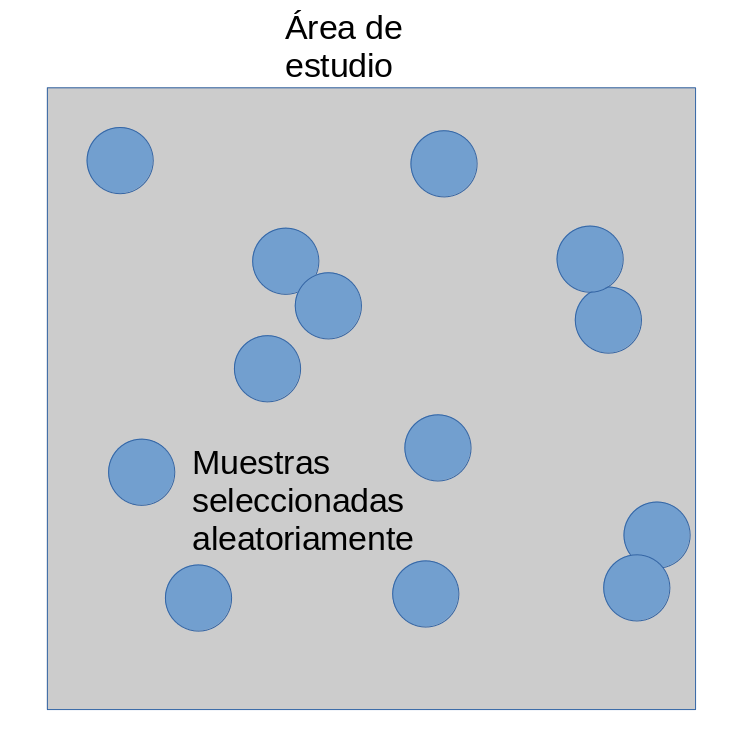
\includegraphics{Figuras-tecnicas/Simple-aleatorio.png}
\end{frame}

\begin{frame}{Estratificado}
\protect\hypertarget{estratificado}{}
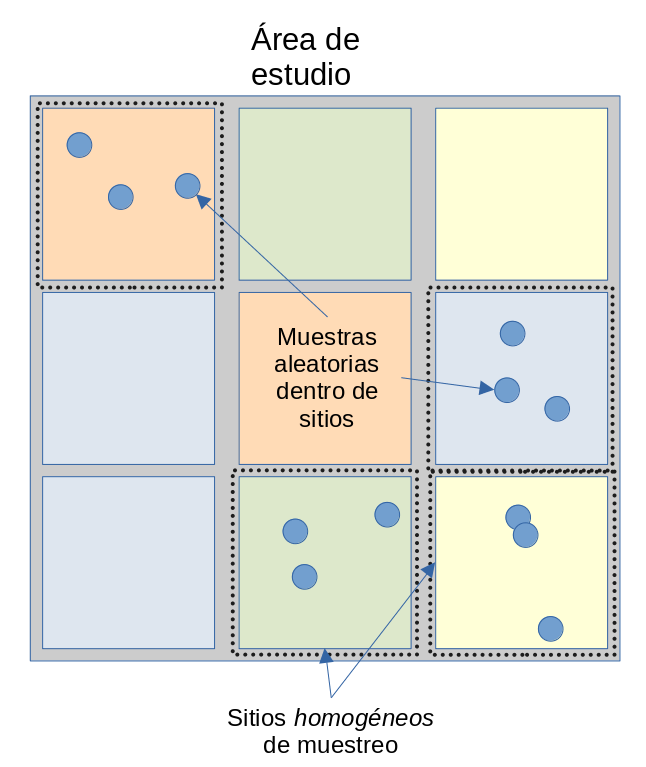
\includegraphics{Figuras-tecnicas/Estratificado.png}
\end{frame}

\begin{frame}{Características}
\protect\hypertarget{caracteruxedsticas}{}
\begin{itemize}
\item
  Muestras más representativas
\item
  Ejemplos en ciencias ambientales y sociales, selección de sitios para
  entrevistas.
\end{itemize}
\end{frame}

\begin{frame}{Agregado (Clúster)}
\protect\hypertarget{agregado-cluxfaster}{}
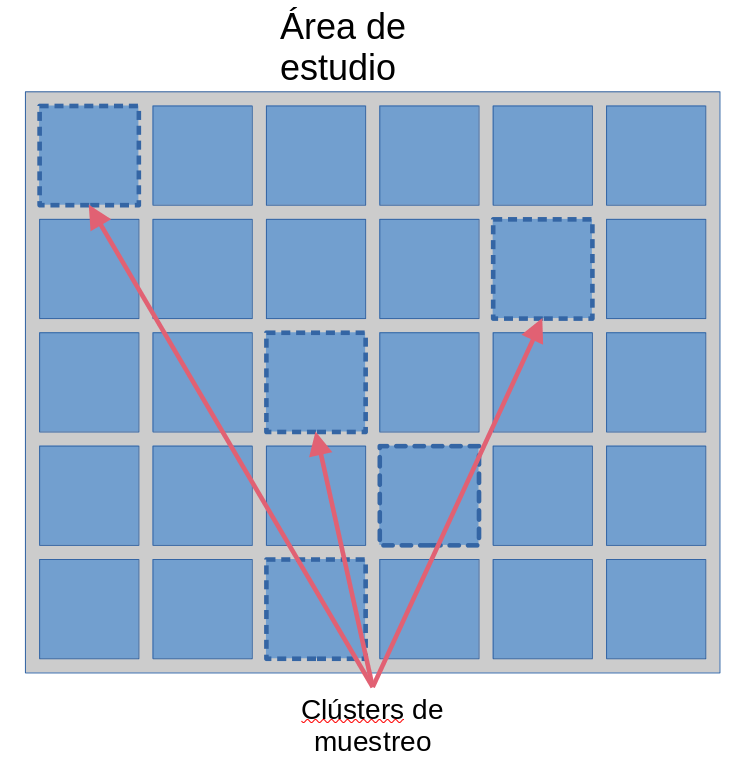
\includegraphics{Figuras-tecnicas/Cluster.png}
\end{frame}

\begin{frame}{Características}
\protect\hypertarget{caracteruxedsticas-1}{}
\begin{itemize}
\item
  En cada clúster se hace un censo
\item
  Sesgos locales muy evidentes
\item
  Ejemplos en estudios demográficos y preferencias electorales
\end{itemize}
\end{frame}

\begin{frame}{Sistemático}
\protect\hypertarget{sistemuxe1tico}{}
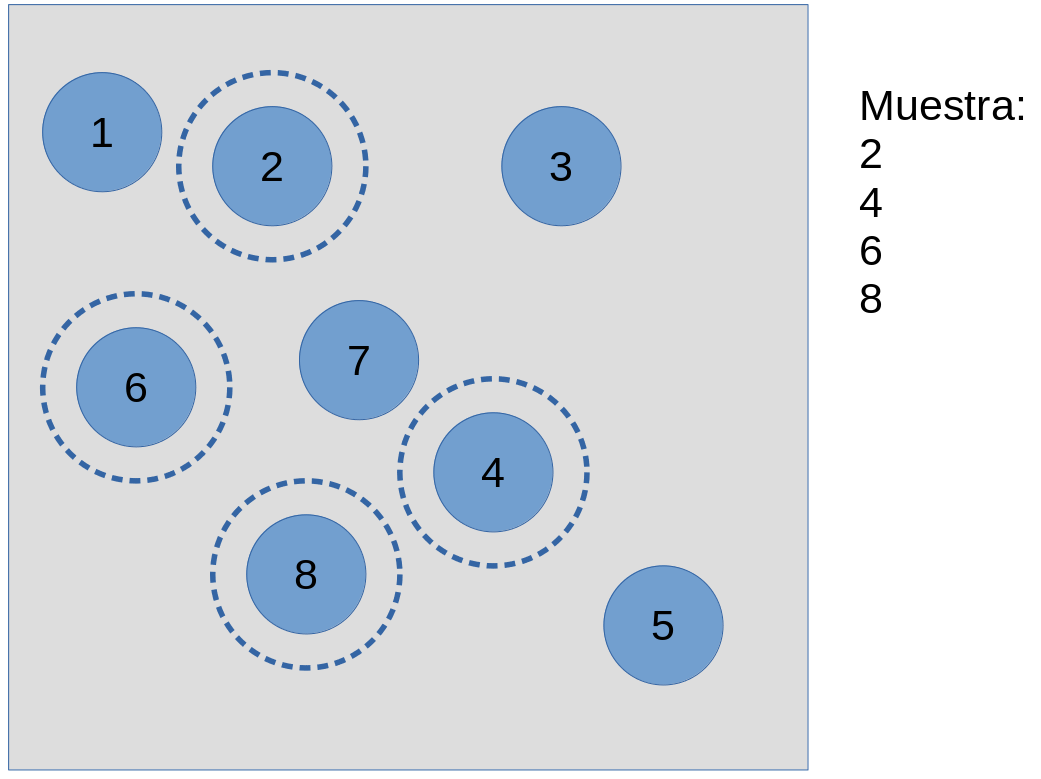
\includegraphics{Figuras-tecnicas/Sistematico.png}
\end{frame}

\begin{frame}{Conveniencia}
\protect\hypertarget{conveniencia}{}
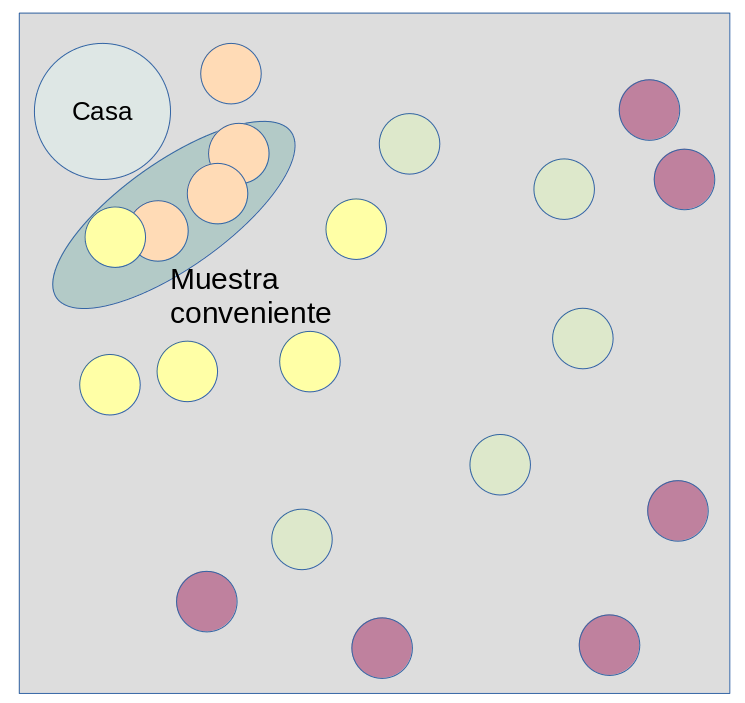
\includegraphics{Figuras-tecnicas/Conveniencia.png}
\end{frame}

\begin{frame}{Características}
\protect\hypertarget{caracteruxedsticas-2}{}
\begin{itemize}
\item
  Es el más sencillo

  \begin{itemize}
  \tightlist
  \item
    Se obtiene muestra de lo más conveniente
  \end{itemize}
\item
  Sesgo muy alto
\end{itemize}
\end{frame}

\end{document}
